\documentclass{amsart}

%--- Paper Size Toggle (uncomment desired size) ---
\newif\ifletter
%\lettertrue % Uncomment this line for Letter size
\letterfalse % Uncomment this line for A4 size

\ifletter
    \usepackage[letterpaper,top=0.8cm,bottom=0.8cm,left=0.8cm,right=0.8cm]{geometry}
\else
    \usepackage[a4paper,top=0.8cm,bottom=0.8cm,left=0.8cm,right=0.8cm]{geometry}
\fi
%-------------------------------------------------

\usepackage{siunitx}
\usepackage{tikz}
\usetikzlibrary{calc}
\usepackage{pgfplots}
\pgfplotsset{compat=1.3}

% --- CONFIGURABLE VARIABLES ---
% Frequency axis
\def\xmin{1e-3}
\def\xmax{1e4}

% Magnitude axis
\def\yminMag{-20}
\def\ymaxMag{400}
\def\ytickstepMag{20}
\def\minorTickNumMag{1}

% Phase axis
\def\yminPhase{-180}
\def\ymaxPhase{180}
\def\ytickstepPhase{45}
\def\minorTickNumPhase{3}
% --------------------------------

\begin{document}
\thispagestyle{empty}
\begin{figure}
    \centering
    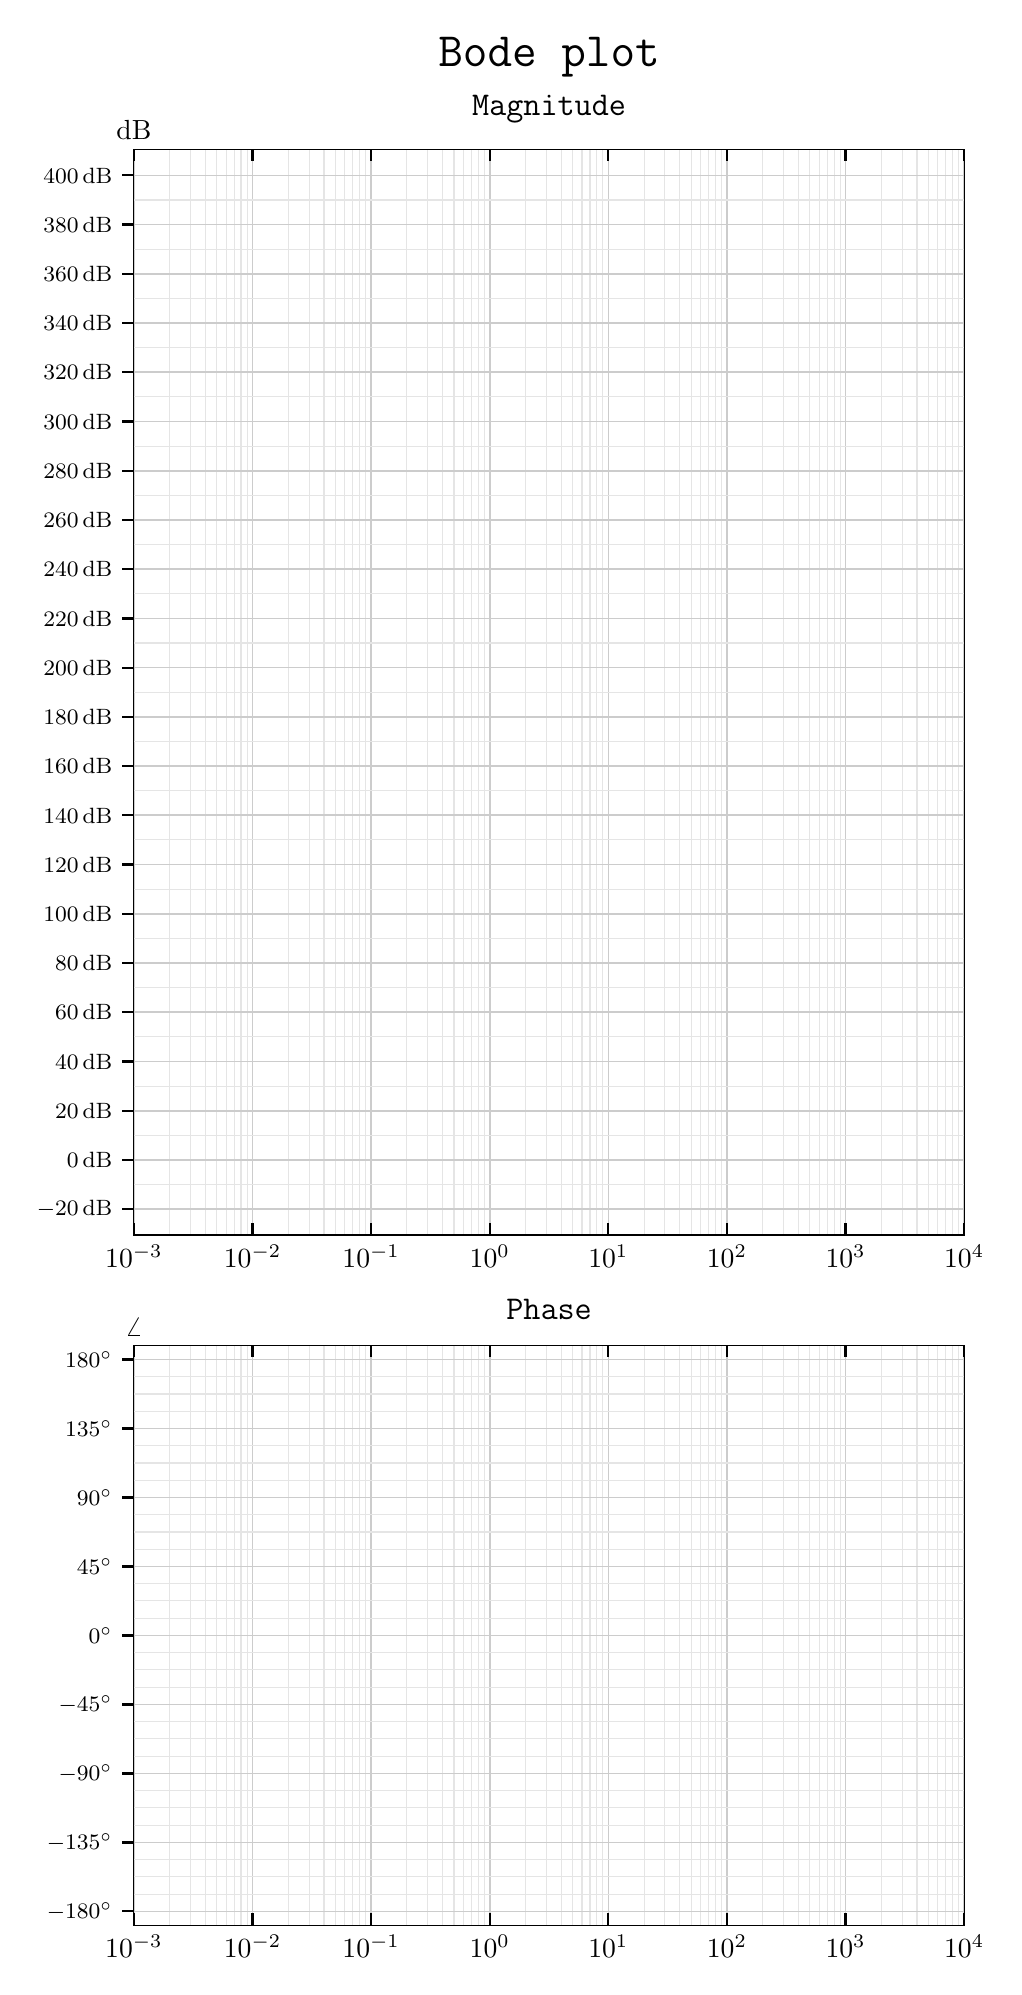
\begin{tikzpicture}
        \begin{axis}[
            name=magnitude,
            title={\texttt{\large{Magnitude}}},
            width=1.0\linewidth,
            height=0.55\paperheight,
            xmode=log,
            ymode=linear,
            axis line style={latex-latex},
            xlabel={},
            ylabel={\si{\decibel}},
            ylabel style={rotate=-90,at={(ticklabel* cs:1)},anchor=south},
            xmin=\xmin, xmax=\xmax,
            ymin=\yminMag, ymax=\ymaxMag,
            enlarge y limits=0.025,
            ytick align=outside,
            ytick pos=left,
            minor tick length=0pt,
            ytick={\yminMag,\numexpr\yminMag+\ytickstepMag\relax,...,\ymaxMag},
            yticklabel style={
                /pgf/number format/.cd,
                fixed,
                precision=0,
                /tikz/.cd,
                font=\footnotesize,
            },
            yticklabel={\pgfmathprintnumber{\tick}\,dB},
            grid=both,
            minor tick num=\minorTickNumMag,
            grid style={line width=.4pt, draw=gray!20},
            minor tick style={line width=.4pt, draw=gray!20},
            major tick style={line width=.8pt,draw=black},
            major grid style={line width=.6pt,draw=gray!40},
        ]
        \end{axis}

        \begin{axis}[
            name=phase,
            title={\texttt{\large{Phase}}},
            at={($(magnitude.south)-(0,40)$)},
            anchor=north,
            width=1.0\linewidth,
            height=0.32\paperheight,
            xmode=log,
            ymode=linear,
            axis line style={latex-latex},
            xlabel={},
            ylabel={$\angle$},
            ylabel style={rotate=-90,at={(ticklabel* cs:1)},anchor=south},
            xmin=\xmin, xmax=\xmax,
            ymin=\yminPhase, ymax=\ymaxPhase,
            enlarge y limits=0.025,
            ytick align=outside,
            ytick pos=left,
            minor tick length=0pt,
            ytick={\yminPhase,\numexpr\yminPhase+\ytickstepPhase\relax,...,\ymaxPhase},
            yticklabel style={
                /pgf/number format/.cd,
                fixed,
                precision=0,
                /tikz/.cd,
                font=\footnotesize,
            },
            yticklabel={\pgfmathprintnumber{\tick}$^\circ$},
            grid=both,
            minor tick num=\minorTickNumPhase,
            grid style={line width=.4pt, draw=gray!20},
            minor tick style={line width=.4pt, draw=gray!20},
            major tick style={line width=.8pt,draw=black},
            major grid style={line width=.6pt,draw=gray!40},
        ]
        \end{axis}

        \node[above,font=\large\bfseries] at ($(magnitude.north)+(0,0.8)$) {\texttt{\LARGE{Bode plot}}};
    \end{tikzpicture}     
\end{figure}
\end{document}
